\documentclass{article}
\usepackage[utf8]{inputenc}
\usepackage[spanish]{babel}
\usepackage{listings}
\usepackage{graphicx}
\graphicspath{ {images/} }
\usepackage{cite}

\begin{document}

\begin{titlepage}
    \begin{center}
        \vspace*{1cm}
            
        \Huge
        \textbf{Taller}
            
        \vspace{0.5cm}
        \LARGE
        Nociones de la memoria del computador
            
        \vspace{1.5cm}
            
        \textbf{Juan Alberto Pineda Montoya}
            
        \vfill
            
        \vspace{0.8cm}
            
        \Large
        Despartamento de Ingeniería Electrónica y Telecomunicaciones\\
        Universidad de Antioquia\\
        Medellín\\
        Septiembre de 2020
            
    \end{center}
\end{titlepage}

\tableofcontents

\section{Introducción}
En este trabajo se presentaran las nociones de la memoria del computador, brindando la definición de la misma, de igual forma se ampliara una visión de sus funciones y las clasificaciones de los diferentes tipos de memorias que existen, así mismo explicando la importancia de las tareas que cumplen.

\section{La memoria} \label{contenido}
\subsection{definición}
La memoria del computador es el dispositivo que se encarga de almacenar la información que circula por el computador, para luego ser utilizada en diferentes procesos.\cite{Augusto}
\subsection{tipos de memorias}
 Existen diferentes tipos de memorias que se utilizan en las computadoras, estos son algunos de ellos:
\subsubsection{disco duro}
El disco duro (HDD hard drive disk por sus siglas en inglés) es un tipo de memoria denominado no volatil ya que almacena información aun estando apagado, es una de las partes más importantes del computador ya que almacena el sistema operativo y la información más valiosa para el correcto funcionamiento del computador.
\begin{figure}[h]
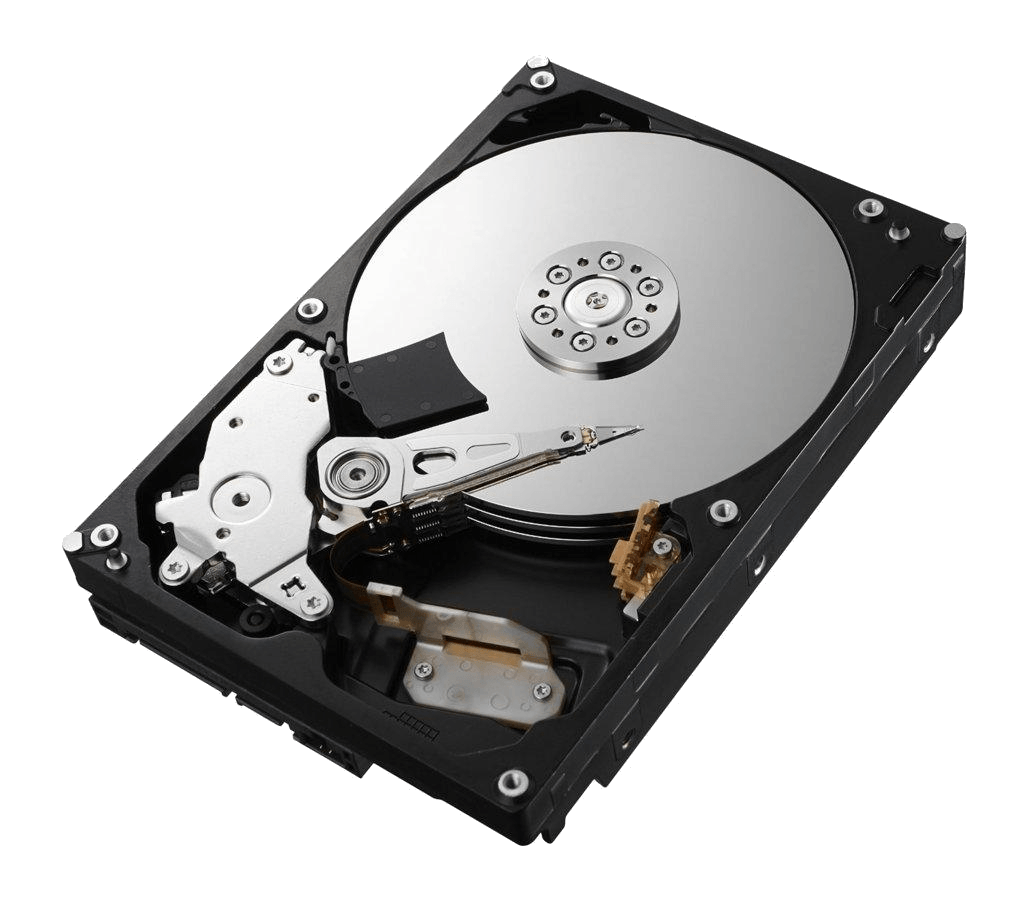
\includegraphics[width=7cm]{hdd.png}
\centering
\caption{disco duro}
\label{fig:HDD}
\end{figure}
\subsubsection{RAM}
La RAM o memoria de acceso aleatorio es una memoria de tipo volátil, ya que almacena información unicamente cuando dispone de corriente, se encarga de guardar las instrucciones de varios componentes del equipo, como por ejemplo de la unidad de procesamiento central.\cite{Edwin}
\begin{figure}[h]
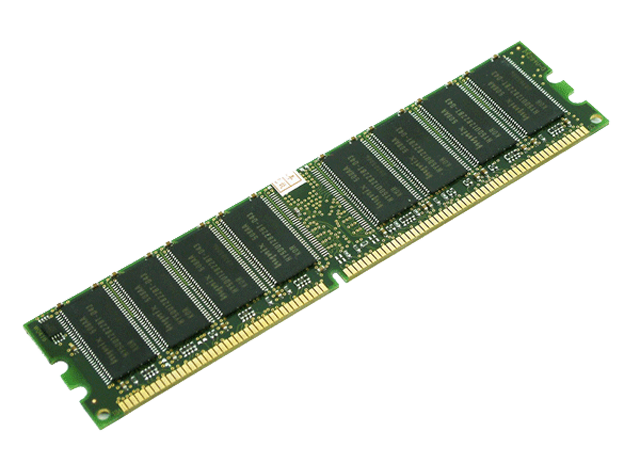
\includegraphics[width=6cm]{RAM.png}
\centering
\caption{RAM}
\label{fig:RAM}
\end{figure}
\subsubsection{ROM}
Memoria de solo lectura, es una memoria que unicamente permite la lectura de información y no permite la escritura, es no volátil, usualmente se usa para almacenar el firmware u otra información de vital importancia para el computador.
\begin{figure}[h]
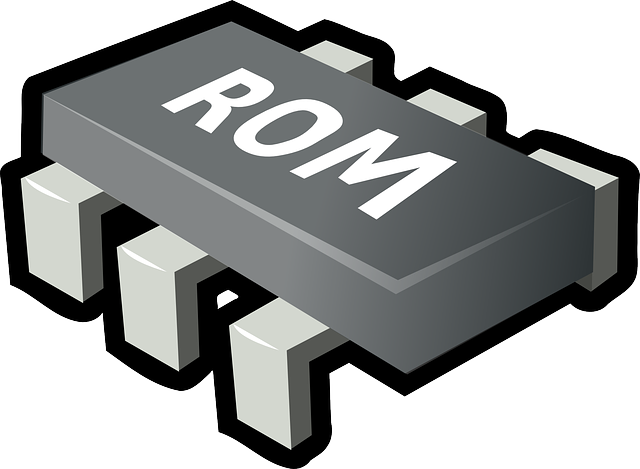
\includegraphics[width=6cm]{ROM.png}
\centering
\caption{ROM}
\label{fig:ROM}
\end{figure}
\subsubsection{Caché}
Es una memoria que guarda datos que se solicitan, para entregarlos de una manera veloz,la lectura del caché es más rápido que realizar nuevamente el cálculo para obtener los datos que ésta ya guardó.
\subsubsection{VRAM}
La VRAM es una memoria de acceso aleatorio dedicada exclusivamente a almacenar contenidos gráficos, como texturas o poligonos.

\subsection{Gestión de la memoria}
La memoria del computador se gestiona a traves de un controlador al cuál se conectan mediante el bus, dicho controlador dictamina el ritmo de las operaciones que se realiza, dando así un orden y gestionando los recursos, a traves del bus se envian y reciben datos que permiten el control de los datos, que serían tres: bus de control, bus de direcciones y bus de datos.
\subsection{velocidad de las memorias}
la velocidad de una memoria se ve definida principalmente al papel que cumplira dentro de la gerarquía de almacenamiento, que se organiza en velocidad, capacidad y costo, donde los metodos mas caros y rápidos, ocupan los niveles más altos y los más lentos, menos caros y de mayor capacidad, los niveles inferiores, siendo el caché de 
CPU el nivel más alto, por su alto costo y gran velocidad, seguido de la RAM, que tiene una gran velocidad y un almacenamiento relativamente alto y por último se encuentra el disco duro, que no es tan rápido, pero es de bajo costo y una capacidad muy amplia. Es importante que exista esta diferencia de velocidad para que la gerarquía de memoría se mantenga correctamente y los datos e información se gestionen debidamente y permitan el funcionamiento del computador.\cite{geniolandia}



\section{Conclusión} \label{conclulsion}
La memoria es un componente esencial y complejo para el funcionamiento correcto del computador, ameritando así, gran cuidado y volviendose un conocimiento casi obligatorio para todo aquel que trabaje en un ambito donde sea muy utilizado.

\bibliographystyle{IEEEtran}
\bibliography{references}

\end{document}
